\documentclass[12pt, a4paper]{article}

\usepackage{graphicx}
\usepackage[utf8]{inputenc}
\usepackage[italian]{babel}
\usepackage{hyperref}

%settings dei links
\hypersetup{
	colorlinks=true,
	linkcolor=black,
	urlcolor=blue,
	pdftoolbar=true,
	pdfmenubar=true,
	pdftitle={AC Torre Archimede},
	pdfauthor={Retis Edoardo},
	pdfcreator={Retis Edoardo}
}

\begin{document}

\frenchspacing
\begin{titlepage}
	\centering
	
\includegraphics[width=0.50\textwidth]{img/logo_unipd_color.png}\par\vspace{1cm} %logo
	
	{\LARGE\bfseries Progetto di Tecnologie Web \par}
	\vspace{1cm}
	
	{\Large\bfseries a.a. 2021/2022 \par}
	\vspace{1.5cm}
	
	{\Large Titolo della pagina web: \par}
	\vspace{0.5cm}
	
	{\LARGE\bfseries\itshape AC TORRE ARCHIMEDE \par}
	
	\vfill 

	Membri del gruppo: \par
	{\bfseries Marco \par}
	{\bfseries Michele \par}
	{\bfseries Stefano \par}
	{\bfseries Edoardo \par}
	
	\vfill

	Indirizzo del sito: \par
	\url{}
	\vfill
	
	% Bottom of the page
	{\large \today\par}
	
\end{titlepage}

%indice
\tableofcontents 
\pagebreak

\section{Introduzione}
Con questo progetto ci poniamo di illustrare un'applicazione web dedita alla promozione delle attività sportive di una associazione calcistica con il fine ultimo di far acquistare dei biglietti per i vari eventi sportivi.\par
La nostra applicazione si pone di soddisfare due obiettivi: il primo è mostrare all'utente tutte le informazioni che riguardano la società, il secondo è dare agli stessi strumenti semplici per poter facilmente avere accesso agli eventi e alle gare della squadra di calcio e prenotare i biglietti per assisterli.\par
Il nostro sito web contiene pagine per visualizzare la storia della società, le recenti notizie pubblicate e la rosa della squadra di calcio; altre sono destinate al calendario delle partite e all'acquisto dei biglietti per lo stadio.

\section{Analisi preliminare del progetto}

\subsection{Requisiti funzionali del sito}
Uno dei requisiti che abbiamo pensato per la nostra applicazione web è avere delle pagine web che forniscano informazioni chiare e precise e che le informazioni siano organizzate in maniera semplice ed esaustive, concentrandoci sugli aspetti che potessero
non solo dare all'utente la risposta che cerca, ma anche di fornire un modo chiaro per farlo. A tal proposito, abbiamo progettato il sito con un design semplice ed intuitivo, concentrandoci di piu' sull'organizzazione del contenuto piuttosto della grafica, rimanendo su una grafica semplice e non invasiva, ma
non per questo da ritenersi obsoleta.\par
Un altro requisito importante per il nostro sito è avere una navigabilità che eviti che l'utente non si disorienti troppo all'interno del sito web e contemporareamente permetta ad esso di trovare facilmente quello che cerca. A tal proposito, è stato implementato
una barra della navigazione semplice e poco profonda e che abbia pagine web suddivise in argomenti ben specifici.\par
Oltre alla navigabilità, si vuole permettere alle persone con disabilità di accedere facilmente alle informazioni del sito web. Un occhio di riguardo è stato fatto anche per l'accessibilità del sito web
seguendo gli standard per l'accessibilità e implementando strumenti utili per utenti che utilizzano gli Screen Reader per navigare su internet.\par
Inoltre, all'interno del sito, l'utente avrà la possibilità di selezionare da una lista di gare quella che preferisce e acquistare l'apposito biglietto. Tali biglietti verranno salvati e visualizzati in una pagina dedicata all'utente.\par

\subsection{Analisi dell'utenza}
Secondo un'analisi preliminare dell'utenza, si è stimata che la maggior affluenza di utenza del sito deriva da tifosi e fan della squadra descritta dal sito. Dato che la tifoseria di una squadra di calcio può essere di tutte le età e di tutti i generi, si e pensato di organizzare le informazioni
per permettere al sito di poter essere usufruibile da un grande bacino eterogeneo di utenti.\par
Dato che si presuppone che la società calcistica abbia sede in Italia e che si assume che la tifoseria della squadra sia italiana, la lingua utilizzata è principalmente l'italiano con qualche termine inglese di comune utilizzo in ambito web (ad esempio, "Password", "Login", "Logout", "News", "Home").
Inoltre, sempre le stesso motivo, non è stato ritenuto necessario implementare più siti web per localizzare il sito in altri paesi oppure per internazionalizzare il sito e non è stato ritenuto necessario aggiungere più lingue.\par
Si è stimato anche che la maggior parte dell'utenza possa accedere al nostro sito tramite dispositivi mobili. Come verrà spiegato nel capitolo dedicato, si è pensato di rendere il nostro sito con design responsivo per poter essere visualizzato da più dispositivi diversi.

\subsection{Attori}
Sono stati individuati tre tipi di attori:

\begin{itemize}
	\item \textbf{Utente non loggato}: egli può usufruire tutti i contenuti del sito, ma non può acquistare nessun biglietto. L'utente non registrato può effettuare un login o creare un nuovo utente dalle apposite pagine, diventando così un utente registrato.
	\item \textbf{Utente loggato}: egli può usufruire tutti i contenuti del sito e può acquistare in base alla gare scelta tra quelle disponibili. Può visualizzare la sua pagina profilo contenente i suoi dati anagrafici e l'elenco delle sue prenotazioni. Può cambiare la propria password ed effettuare il logout, diventando così un utente non loggato.
	\item \textbf{Amministratore}: egli ha gli stessi permessi che possiede un utente loggato, ma ha a disposizione anche un area riservata dove può gestire gli articoli e l'elenco delle gare all'inteno del sito.
\end{itemize}

\subsection{Analisi della base informativa}
Il gruppo ha prodotto quasi interamente i contenuti presenti nel sito. All'interno del sito, troviamo le informazioni divise da due tipologie di organizzazione: le informazioni organizzate sotto forma di descrizione e l'altra sotto forma di tabelle.\par
La prima tipologia di organizzazione serve per aree del sito (ad esempio, Stadio) dove che bisogno di descrivere in maniera precisa ed esaustiva un argomento specifico per poter essere facilmente compreso dalla maggior parte dell'utente. Dentro queste descrizioni possono esserci anche immagini di contorno per abbellire la pagina e non avere un semplice muro di testo.
Per queste immagini non serve mettere testo alternativo in quanto gli screen reader non devono leggere queste immagini.\par
La seconda tipologia di organizzazione serve per aree (ad esempio, Calendario) dove si ha la necessità di organizzare molti record di informazioni dentro un'unica tabella. Si è cercato di rendere le tabelle accessibili per dare la possibilità agli screen reader di poterle leggere con semplicità e si è studiato una soluzione anche di poterle farle visualizzare a tutti i dispositivi mobili, 
migliorando l'usabilità del sito.

\section{Organizzazione del lavoro}

\subsection{Divisione dei compiti}
Al momento della conformazione del gruppo, ogni componente ha potuto decidere quale parte del progetto avrebbe preferito curare e realizzare.
Il lavoro è stato così suddiviso:

\begin{itemize}
	\item Marco:
	\item Michele:
	\item Stefano:
	\item Edoardo:
\end{itemize}

Per quanto riguarda la condivisione del materiale è stata usata la piattaforma di \texttt{GitHub}. La 
repository è raggiungibile al seguente link: \url{https://github.com/markio00/tecweb_AC-TorreArchimede}.

\subsection{Tempistiche}

\pagebreak

\section{Tecnologie}

\pagebreak

\section{Progettazione}

\subsection{Schema e struttura organizzativa del sito}
Durante la progettazione del sito, è stato deciso di organizzare le varie aree per topic, dove in ogni sezione del sito le varie informazioni sono raggruppate
per uno specifico argomento. Questa decisione, anche se comporta la difficile mantenibilità del sito, perchè deve essere sempre in costante aggiornamento, è stata presa perchè permette all'utente
di trovare facilmente le informazioni che cerca, specialmente quando esso non sa esattamente cosa si sta cercando, aiutando molto la navigabilità del sito.\par
Il nostro sito web è suddiviso nelle seguenti sezioni:
\begin{itemize}
	\item \textbf{Home}: è la "\textit{vetrina}" del nostro sito. Dentro questa sezione l'utente può trovare informazioni di vario genere e che rappresentano tutto quello che si può trovare o
	cercare nel sito e vari collegamenti ipertestuali per permettere all'utente di saltare subito alla pagina che si vuole visualizzare.
	\item \textbf{News}: è la sezione dove vengono visualizzate tutte le notizie e articoli che riguardano l'attività sportiva della società calcistica. Per evitare il sovraccarico cognitivo, sono stati aggiunti degli indici
	che si aggiornano dinamicamente per visualizzare solo una parte delle notizie caricate dall'admin, ma l'utente le può scorrere usando i suddetti indici.
	\item \textbf{Stadio}: è la sezione dove vengono raggruppate tutte le informazioni sulla storia dello stadio della società rappresentata dal sito. Contiene contenuto puramente informativo.
	\item \textbf{La Squadra}: è la sezione dove viene visualizzato l'elenco dei calciatori e dei tecnici della squadra di calcio. Anche qua, il contenuto è puramente informativo.
	\item \textbf{calendario}: è la sezione dove sono elencate le ultime gare disputate dalla squadra. Essendoci una tabella, abbiamo sviluppato la sezione tenendo conto di rendere la tabella accessibile per tutti i dispositivi.
	\item \textbf{Biglietteria}: è la sezione dove sono elencate le prossime gare che la squadra andrà a disputare. In questa sezione, oltre ad avere informazioni puramente informative, ha anche dei collegamenti ipertestuali per 
	permettere all'utente di raggiungere la pagina \textit{checkout}, dove l'utente ha la possibilità di acquistare il biglietto scelto. Come per la precedente sezione, abbiamo tenuto conto che la tabella deve essere accessibile
	per tutti i dispositivi.
	\item \textbf{login}: è la sezione dove l'utente può loggarsi al sito. Se si logga correttamente, l'utente viene indirizzato nella propria \textit{area personale}, altrimenti ci sono link utili per registrarsi oppure per 
	recuperare la propria password nella sezione \textit{Recupera password}.
	\item \textbf{Area personale/Area admin}: è la sezione dove un utente loggato può visualizzare e gestire i propri dati anagrafici e l'elenco dei biglietti acquistati. Se l'utente loggato è un amministratore del sito, questa sezione
	avrà al suo interno un area riservata a soli admin, dove essi posso aggiungere e gestire gli articoli visualizzati nella sezione \textit{News} e le gare visualizzate nelle sezioni \textit{Calendario} e \textit{Biglietteria}.
	Come per le sezioni precedenti, le tabelle visualizzate in questa sezione devono essere accessibili.
	\item \textbf{Registrazione}: è la sezione dove un utente non registrato potrà inserire i propri dati personali in un apposita form per poter registrarsi la sito e avere dunque la possibilità di loggarsi al sito e usufruire
	dell'area personale.
\end{itemize}

Come struttura organizzativa del sito, abbiamo implementato una struttura a gerarchia con suddivisioni mutualmente esclusive con un ampiezza di opzioni di 7 pagine e una profondita di livelli di massimo 2 livelli.
E' stata fatta questa scelta per migliorare la navigabilità del sito, inserendo tutte le opzioni all'interno della barra di navigazione principale del sito, permettendo così di rendono gli utenti in grado di sviluppare facilmente un modello 
mentale della struttura del sito e della loro localizzazione in questa struttura. Inoltre, è stata fatta questa scelta anche per permettere al sito di essere facilmente aggiornato ed evoluto.

\begin{figure}[htb]
	\centering
	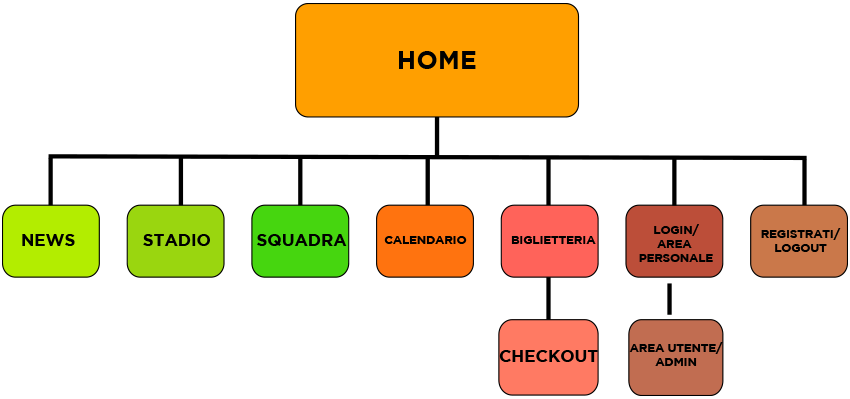
\includegraphics[width=10cm]{img/schema_sito.png}
	\caption{Immagine che mostra la struttura gerarchica del sito.}
\end{figure}

\pagebreak

\subsection{Struttura delle pagine}
Tutte le pagine principali utilizzano il seguente schema:
\begin{itemize}
	\item \textbf{Header}: dove sono presenti logo e titolo della pagina web;
	\item \textbf{menu'}: indica quali pagine possono essere navigate e comunica se l'utente è loggato oppure no;
	\item \textbf{Path}: indica dove ci troviamo all'interno del sito;
	\item \textbf{Corpo}: contiene i contenuti della pagina;
	\item \textbf{Footer}: utilizzato per inserire i loghi della validazione forniti da w3c.
\end{itemize}

Per l'organizzazione delle pagine, è stato scelto di utilizzare un layout verticare per rispettare le convenzioni esterne della maggior parte degli utenti
e facilitare la gestione di un design piu' responsivo per quando si naviga utilizzando dispositivi diversi dal PC (vedi paragrafo Presentazione/CSS).

\begin{figure}[htb]
	\centering
	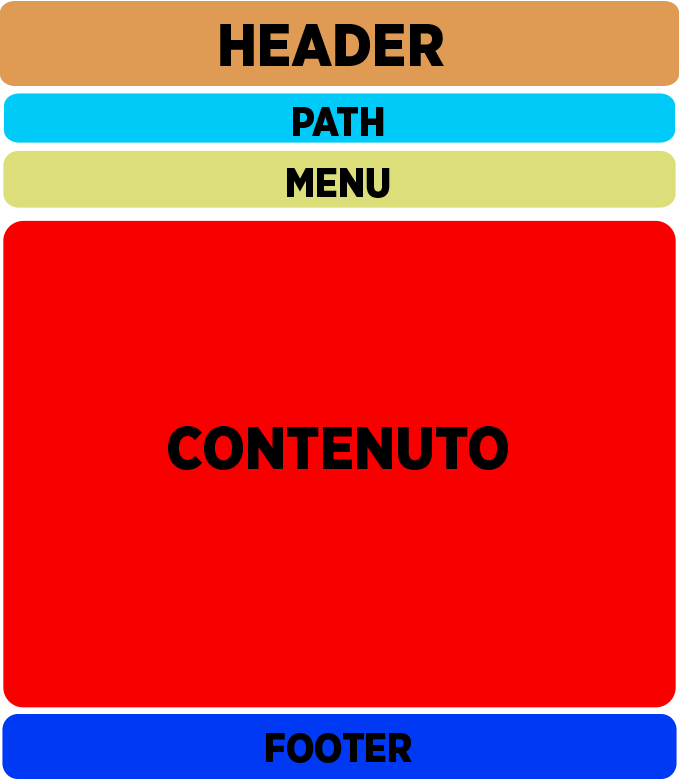
\includegraphics[height=9cm]{img/schema_pagina.png}
	\caption{Immagine che mostra il design del layout scelto.}	
\end{figure}

\section{Costruzione del sito}

\subsection{Separazione tra struttura, presentazione e comportamento}
Il nostro gruppo di lavoro ha basato l'intera costruzione del sito sul principio di sepazione tra struttura, presentazione e comportamento. All'interno della repository su Github, abbiamo organizzato i vari file di codice per l'implementazione del sito in quattro
cartelle \textit{html}, \textit{css}, \textit{php} e \textit{js}, contenenti rispettivamente file HTML, CSS, PHP e Javascript. La scelta di questo principio stà nel rendere il codice più mantenibile possibile e di facile modifica. Inoltre, tale separazione rende il sito
internet più leggero in termini di spazio occupato a memoria nel server.

\subsection{Struttura}
Nella cartella \textit{html}, sono presenti file .html contenti presets per impaginare le varie pagine web e pezzi di codice html per costruire il corpo di ogni pagina del sito.
Tutti questi file verranno usati dai vari file .php per costruire la pagina vera e propria. Tutte i file .html hanno al loro interno dei placeholders contrassegnati da una coppia di percentuali. Essi vengono usati
dal codice PHP per generare dinamicamente codice HTML, il contenuto ed eventuali errori da mostrare nelle varie pagine.\par
I file \texttt{head.html}, \texttt{navbar.html} e \texttt{footer.html} sono i presets che vengono usati per generare in ogni pagina rispettivamente l'intestazione della pagina con il tag \texttt{<head>} e tutti i tag \texttt{<meta>}
da inserire, il titolo del sito web, la barra di navigazione e il breadcrumb da inserire prima del contenuto e il piè di pagina con tutte le informazioni sui sviluppatori. In più, all'interno della cartella \textit{tables} ci sono vari presets contenenti le intestazioni dell varie tabelle del sito
e un file \texttt{struttura.html} contenente dei placeholders per generare una singola tabella.
Invece, tutti gli altri file contenuti nella medesima cartella contengono il corpo di ogni pagina. Ecco l'elenco dei file con una breve descrizione:
\begin{itemize}
	\item \texttt{index.html}: è il corpo della Home contenente un tag \texttt{<aside>} per mostrare un anteprima delle prime news visualizzate nell'apposita pagina.
	e tre tag \texttt{<section>} contenenti anteprime delle prossime gare, della storia dello stadio e della rosa dei calciatori e all'interno di questi tag sono presenti link che rimandano alle rispettive pagine web.
	Per visualizzare la tabella delle partite in questa pagina, è stato utilizzato un preset chiamato \texttt{home\_header.html}.
	\item \texttt{news.html}: è il corpo della News, ma contiene soltanto 3 placeholders. I vari articoli e gli indici andranno generati dinamicamente in base ai contenuti estratti dal database.
	\item \texttt{stadio.html}: è il corpo della pagina Stadio contenente due paragrafi riguardante la storia dello stadio con le relative immagini di contorno.
	\item \texttt{squadra.html}: è il corpo della pagina La Squadra contenente due liste che sono rispettivamente la lista dei tecnici e dei calciatori della squadra di calcio.
	\item \texttt{calendario.html}: è il corpo della pagina Calendario contenente i placeholders per generare la tabella delle partite disputate. Per generare la tabella, viene usato il preset \texttt{match\_header.html}.
	\item \texttt{biglietteria.html}: è il corpo della pagina Biglietteria contenente i placeholders per generare la tabella delle partite da disputare con i relativi link per acquistare i biglietti. Per generare la tabella, viene usato il preset \texttt{biglietto\_header.html}.
	\item \texttt{checkout.html}: è il corpo della pagina Checkout contenente una form per poter inserire i dati per acquistare i biglietti per la partita selezionata.
	\item \texttt{login.html}: è il corpo della pagina Login contenente una form da copilare per potersi loggare al sito web.
	\item \texttt{dashboard.html}: è il corpo della pagina Area Personale contenente vari placeholders per visualizzare i dati anagrafici dell'utente loggato e le due tabelle che mostrano le partite disputate e le partite da disputare. Per generare le tabelle, vengono usati i preset \texttt{refundable\_ticket.html} e \texttt{ticket\_header.html}.
	\item \texttt{dashboard\_admin.html}: è il corpo della pagina Dashboard Admin contenente una form per aggiungere un nuovo articolo nel database, un bottone per andare alla pagina per aggiungere nuove partite e un placeholder per generare la tabella per gestire le partite inserite nel database. Per generare la tabella, viene usato il preset \texttt{match\_admin\_header.html}.
	\item \texttt{addedit\_match.html}: è il corpo della pagina dell'admin per gestire le partire da inserire nel database contenente una form per inserire i dati della partita.
	\item \texttt{recupero\_password.html}: è il corpo della pagina Recupero password contenente una form per permettere all'utente di cambiare la password dimenticata.
	\item \texttt{signup.html}: è il corpo della pagina Registrazione contenente una form per permettere all'utente di registrarsi al sito web.
\end{itemize}

\subsection{Presentazione}
La presentazione del sito è stata implementata usando quattro fogli di stile CSS, uno per la visualizzazione su schermo desktop (style.css), uno dedicato alla visualizzazione su dispositivi mobili tablet (tablet.css), uno dedicato alla visualizzazione su dispositivi mobili smartphone (mobile.css) ed infine
l'ultimo deidcato alla stampa (print.css). Come suggerisce il principio di suddivisione tra contenuto, struttura e comportamento, questi file si occupano solamente della realizzazione grafica del sito.

\subsubsection{CSS Desktop}
\texttt{style.css} è il foglio di stile principale del nostro sito e crea la grafica per un dispositivo desktop, quali PC o laptop. Il nostro gruppo di lavoro ha scelto di implementare un design elastico che oltre a migliorare l'usabilità tra i vari dispositivi, favorisce anche l'accessibilità. 
Questo foglio di stile permette di visualizzare il logo e l'intestazione del sito utilizzando tutto lo spazio possibile e la barra di navigazione in orizzontale, estendendola su tutto quanto lo schermo. In \texttt{index.php}, l'aside dell'anteprima delle notizie viene visualizzata sulla sinistra dello schermo.\par
Sono state utilizzate misure relative, ovvero gli em e le percentuali, per scrivere le varie regole CSS e il gruppo di lavoro ha cercato di applicare uno stile grafico semplice e chiaro, basato su pochi colori (principalmente, quelli della squadra di calcio) e forme semplici, che favorisce l'usabilità senza rinunciare ad una grafica piacevole.

\subsubsection{CSS Mobile}
In \texttt{tablet.css} vengono definite le regole CSS per i dispositivi con larghezza inferiore a 1061px, mentre in \texttt{mobile.css} vengono definite le regole CSS per i dispositivi con larghezza inferiore a 520px.\par
Nel CSS per i tablet, è stata ridimensionata la lunghezza della barra di navigazione e (così come per il CSS per gli smartphone) l'aside dell'anteprima delle notizie nella homepage è stata spostata al centro come tutte le altre informazioni.
Per quanto riguarda la grafica per i piccoli dispositivi, l'intestazione e la barra della navigazione sono state modificate. Il titolo è stato tolto e al suo posto è rimasto solo il logo, mentre al posto della barra di navigazione, sono stati aggiunti due pulsanti che, se tappati, fanno comparire il menù del login e il menù principale del sito.
Anche le tabelle sono state modificate in favore di un design più verticalizzato. Di seguito, vengono fornite alcune schermate per mostrare i diversi design delle tabelle:

(inserire immagini)

\subsubsection{CSS di stampa}
\texttt{print.css} fornisce il CSS per stampare una pagina del sito. Per creare il foglio di stile, il gruppo di lavoro ha scelto di eliminare tutti gli elementi grafici non strettamente necessari alla comprensione del contenuto o inutili in un foglio stampato (come, ad esempio, la barra di navigazione). Si è scelto il font "\textit{Times New Roman}" adatto alla stampa.\par
Si fornisce un confronto tra lo stile da schermo e lo stile da stampa:

(inserire immagine)





\end{document}
